\documentclass[msc,oneside]{ubcthesis}%msc, phd, masc, ma, or meng

% ================================================================================
% CHANGE THE FOLLOWING ACCORDING TO YOUR PROGRAM/THESIS
% ================================================================================
\institution{The University Of British Columbia}
\program{Computer Science}
\faculty{THE IRVING K. BARBER SCHOOL OF ARTS AND SCIENCES}
\institutionaddress{Okanagan}

% For an Honours thesis, use \documentclasss[msc,oneside]{ubcthesis} above and
% uncomment and modify the next line:
\degreetitle{B.Sc. Computer Science Honours}

\title{The Source}
%\subtitle{With a Subtitle}
\author{Raffi Kudlac} % The name needs to be exactly the same as on the diploma i.e. (Name from SISC)
\copyrightyear{2015}
\submitdate{April 2015} % date of approved thesis
%\program{Interdisciplinary Studies - Optimization}%or Mathematics, or Interdisciplinary Studies
%\previousdegree{B.Sc. Hons., The University of British Columbia, 2008}
%\previousdegree{M.Sc., The University of British Columbia, 2010}

% ================================================================================

\usepackage{ubcostyle} %loads packages
\usepackage{pgf}
\usepackage{siunitx}
\usepackage{longtable}

% ===================================================================
% CHANGE THE FOLLOWING COMMANDS ACCORDING TO YOUR NEEDS
% ===================================================================
\newcommand{\R}{\mathbb{R}}   %real number
\newcommand{\Z}{\mathbb{Z}}   %integers
\newcommand{\C}{\mathbb{C}}   %complex numbers

\sisetup{round-mode=places,round-precision=0}
\newcommand{\percent}[2]{\pgfmathparse{#1*100/#2} \num{\pgfmathresult}\%}

\newcommand{\dom}{\operatorname{dom}}
\providecommand{\TT}[1]{\Theta\left(#1\right)} % big-Theta
\providecommand{\OO}[1]{\mathcal{O}\left(#1\right)} % big-Oh
% ===================================================================

%Uncomment the next line if there are more than one appendix
%\renewcommand*\appendixname{Appendices}


\begin{document}

% This starts numbering in Roman numerals as required for the thesis
% style.
\frontmatter                    % Mandatory

% The order of the following components should be preserved.  The order
% listed here is the order currently required by FoGS.
\maketitle                      % Mandatory

\newpage
\phantomsection \label{tableofcontent}%set anchor at right location
\addcontentsline{toc}{chapter}{\contentsname}
\tableofcontents                % Mandatory: generate toc
\newpage 
\phantomsection \label{listoftab}%set anchor at right location
\addcontentsline{toc}{chapter}{\listtablename}
\listoftables                   % Mandatory if thesis has tables
\newpage
\phantomsection \label{listoffig}%set anchor at right location
\addcontentsline{toc}{chapter}{\listfigurename}
\listoffigures                  % Mandatory if thesis has figures

% Any other unusual prefactory material should come here before the
% main body.

% Now regular page numbering begins.
\mainmatter

% Parts are the largest structural units, but are optional.
%\part{Thesis}

% Chapters are the next main unit.
\chapter{Introduction}
	“The Source” is an interactive simulation model where the user is charged with the task of providing 
energy to a growing population. The purpose of the simulation is to show the benefits and detriments of 
each type of energy source. Although the game targets young adults, primarily around high school and 
College/university students; anyone can play and and have a learning experience. Two intended outcomes of 
the simulation are to demonstrate the ratio of energy output to energy source type, and show the inner 
workings of each. A third outcome of the simulation is show that each type of energy works in the same way 
at its most basic level, with the exception of solar power converting kinetic energy into electrical energy.
\bigskip

The user will accomplish the task of providing energy by choosing to invest in different types of energy. 
The energy types that are at the users' disposal are solar, wind, hydro, coal, oil, gas and nuclear. Users 
can choose to build any of these power plants, but each type has consequences that others may not have. For 
example, if a user decided to build a power plant that ran off of coal, environmentalists would be 
displeased because the burning of coal introduces pollutants into the atmosphere. As well as considering 
the consequences of their actions, the users must also consider what fuels each power plant and how long 
each power plant can be sustained for. Fossil fuels and nuclear power are not infinite; the user must find 
resources to fuel these power plants. Users can choose to invest in renewable resources such as solar, wind 
and hydro, but the problem the user encounters with these types of resources is that they don't output as 
much energy as fossil fuels. The users' main objective is to survive for as long as possible and to beat 
their previous time. 

\chapter{Energy Today}
  In our society, almost all of our energy that powers our homes and businesses is created in the same way. 
It could be argued that Michael Faraday, the inventor of the concept of the generator, had the biggest 
effect on the development of our society. In the early 1800's Faraday discovered that a magnet traveling 
through a coiled wire which could then be redirected 
to wherever energy was needed. This concept is at the core of all our power generation. In the following sections we will cover a few of the different kinds of power and the pros and cons of each. Power is something that everone uses in thier everyday lives and therefor it is important to have even a general understanding of how it works. 

\section{Generators}
  
  All generators operate in the same fashion, transferring kinetic energy into electrical energy. Some generators perform this transfer by having a stationary coil and moving a magnet through the coil as shown in Figure \ref{Induction}, while other generators have stationary magnets and move the coil through the magnetic field generated between two magnets. It does not matter which method is used, the same rules of physics are applied and both ways achieve the result of a flowing current. The faster the movement of the coil or magnet the more current will be generated. 
  The more current that is generated the more power there is to use. Generators have a couple more components to them including, but not limited to, gas chambers and rotating pistons. These components are all just tools used to convert the potential energy of the power source into kinetic energy and finally into the desired electrical energy. This concept is the heart of all major methods of power production.

  \begin{figure}[hbt]{\label{Induction} }
  \begin{center}
    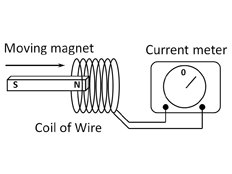
\includegraphics[width=0.3\textwidth]{Induction}
    \caption[Generator Mechanics]{Generator Mechanics \cite{Current}}  
  \end{center}
\end{figure}

\newpage
  \section{Fossil Fuels}

  All Fossil fuel plants operate in the same way; they burn a substance to heat water that is turned into 
  steam and that steam is then fed to flow past a turbine. The steam pushes the turbine which is connected to a generator. This motion feeds kinetic energy to the generator which then turns the energy into electrical energy for people to use. This is shown in Figure \ref{FossilFuelCycle} which specifically shows the process of a coal power plant. 

Fossil fuel plants have one specific difference from each other, which is in the substance that they burn and the different protocols and buildings erected to handle the substances. Other than this difference the process is the same for oil, gas, coal and even nuclear power plants. Once the substance has been burned, the heat is transferred into water. In order to obtain as much energy as possible, the water is kept under pressure making it able to be heated to temperatures much higher then $100^\circ$C. Once the water is at the desired temperature, it is fed through a series of pipes from which it enters another chamber. In this chamber, the water leaves the pipes at extraordinary speeds and is turned into steam instantaneously as the pressure keeping the water in liquid state is released. The fast moving steam pushes against a turbine causing it to move, and in turn, causing the components in the generator to be moved, thus generating a current. 

 \begin{figure}[hbt] \label{FossilFuelCycle} 
    \begin{center}
      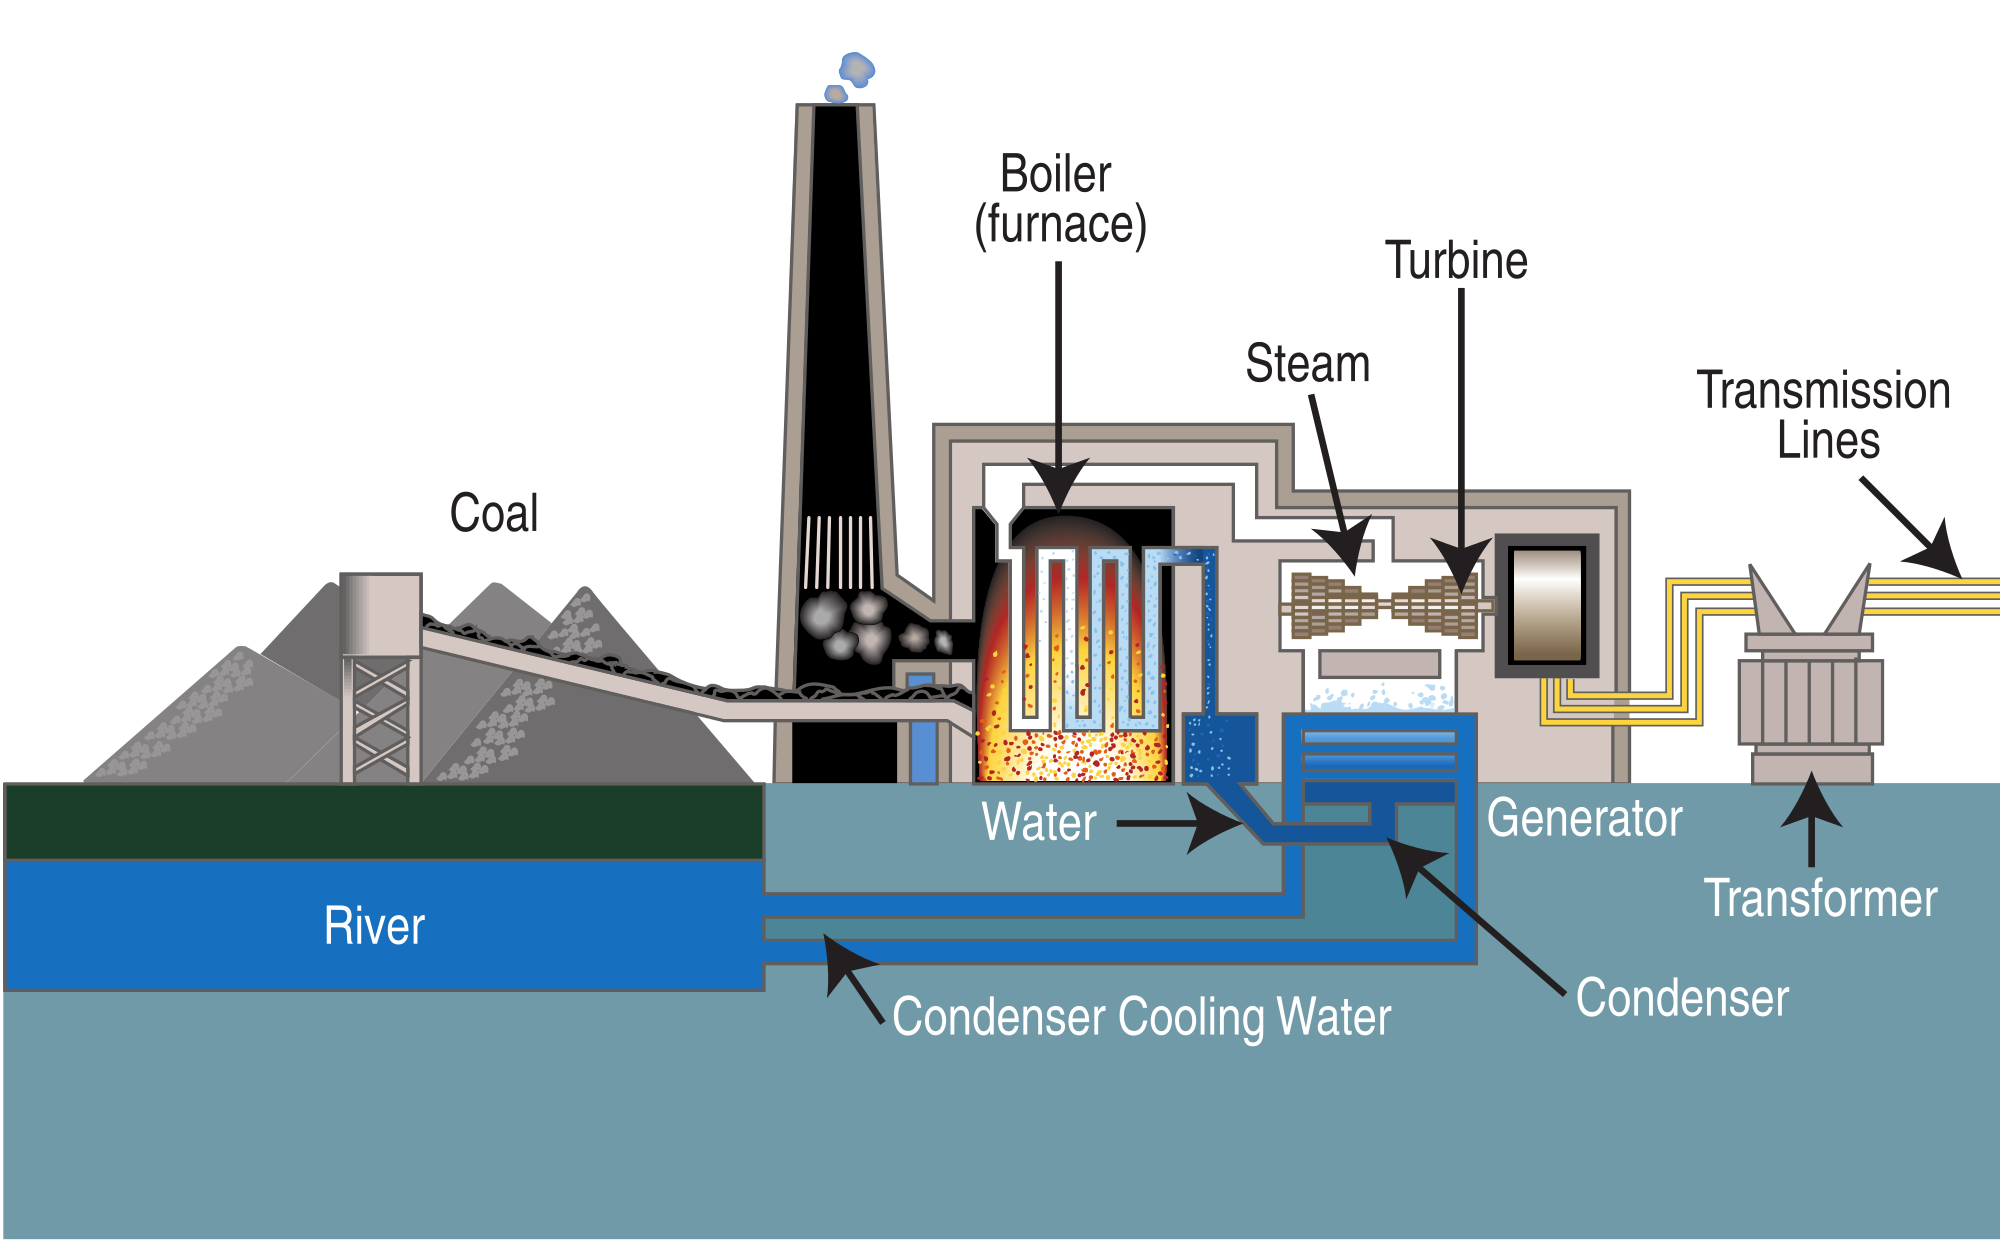
\includegraphics[width=1\textwidth]{fossil_fuel}
      \caption[Fossil Fuel Cycle]{Fossil Fuel Cycle \cite{Coal}}
    \end{center}
  \end{figure}

\newpage

In order to save water, the steam is collected and condensed back into water to be used again. Plants are 
usually built around a water source as water needs to be switched out at times to cool components of the plant. Since plants use water to function it is convientient to have a water source close by. When water gets cycled out of the plant and back into the water source it is warm and can have negative effects on wildlife. Imagine if someone cranked the thermostat in your house to $40^\circ$C, how would you like it?

Fossil fuel power plants generally produce large amounts of power and the price of fossil fuels is generally cheap, but they have huge environmental consequences such as carbon dioxide being produced. Fossil fuel plants also run on a limited resource like coal and once the resource is depleted they will be useless.

 \section{Nuclear Power}

 Nuclear power may be the most desired power source on the planet. Nuclear power is capable of producing tremendous amounts of power for doing little work. All nuclear power plants today run off of fission, the process of breaking up atoms into smaller ones. The element that nuclear plants currently run off of is Uranium. Uranium has nice properties for being broken apart. One property being that large amounts of energy are released when fission occurs and this energy is given off in the form of heat. Just like fossil fuel 
 power plants nuclear power plants operate by taking this heat, heating water into steam, using the steam 
 to turn a turbine and then the turbine turns a generator. This is shown in Figure \ref{nuclearCycle}.

However the process of getting the heat is dramatically different. In the reactor of a nuclear power 
plant there are Uranium rods, that fuel the plant. The rods are bombarded with nuclei that breaks apart the 
Uranium in the rods when it collides with the nuclei. Essentially it is like breaking when playing pool. The cue ball is the nuclei and 
the triangle of pool balls is the Uranium atom. Instead of sound being released when a collision occurs, 
heat gets released. The Uranium rods are surrounded by water and this water absorbs the heat from the 
fission reaction. Just like in fossil fuel power plants, the water is kept under pressure so that it can be 
heated to higher temperatures. Some designs vary but in a pressurized water reactor the water that is in contact with the core can not come in contact with other parts of the plant. This is because this water is radio-active from its contact with the core. It is not 
turned into steam and is instead sent through a series of pipes away from the reactor. This water never 
leaves the pipes but is used to heat more water, safe water, that has outside contact with the pipes. From 
here the process is the same as with fossil fuel power plants.

\begin{figure}[hbt]\label{nuclearCycle}
  \begin{center}
    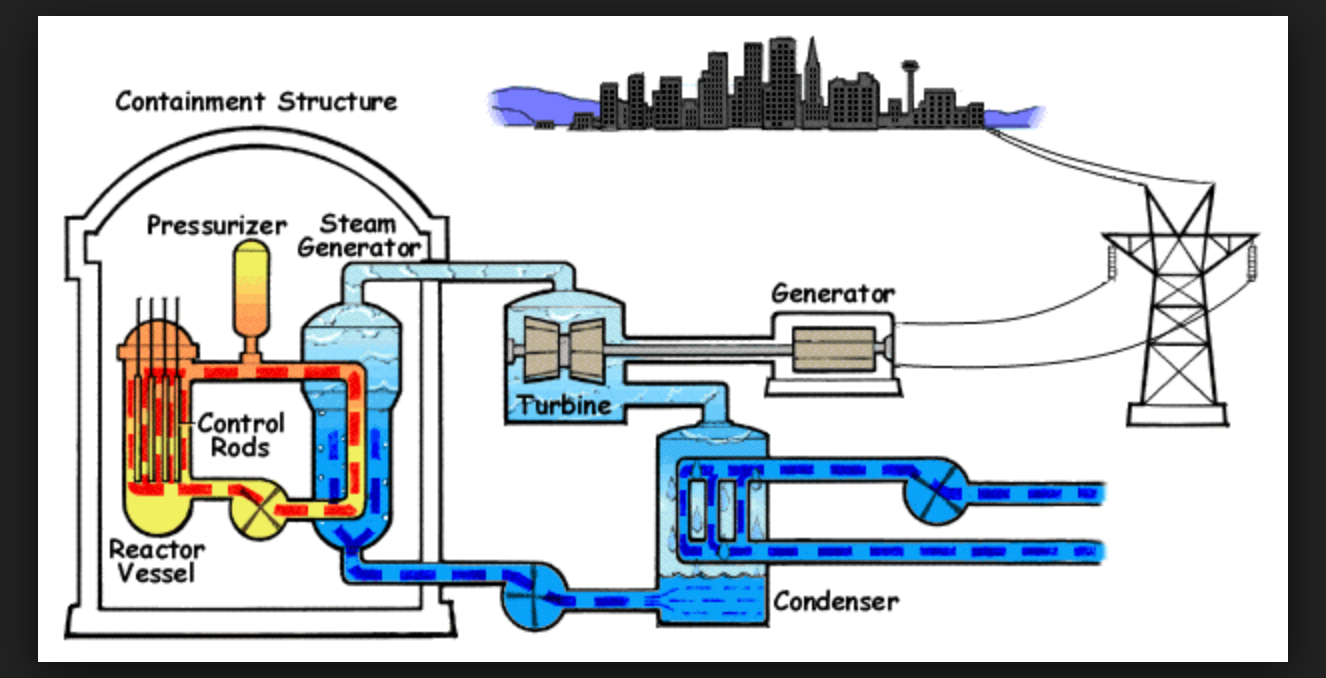
\includegraphics[width=1\textwidth]{nuclear}
    \caption[Nuclear Cycle]{Nuclear Cycle \cite{Nuclear}}
  \end{center}
\end{figure}

Nuclear power plants have little waste compared to fossil fuel plants but they do 
produce radio-active waste (left-overs from the fission reaction). This radio active waste can last for hundreds of years and there is no way to dispose of it other then to leave it on its own. Also It takes energy to mine the Uranium, refine it and transport it to the plant. This process can be lengthy and can leave the earth scared with dig sites. Like fossil fuels, Uranium is a resource found in the Earth's crust and there is a finite amount of it. There is far more uranium than all the fossil fuels combined and we are using it up at a slower rate but one day we will run out and science will have to find a new kind of power source for fission. 
Even with all these draw backs nuclear power is one of the most power abundant method for creating energy. Nuclear plants can power huge populations of people and even though nuclear waste is produced, it is tiny compared to the waste of the other fossile fuels. 

\section{Hydro Power}

Hydro power, arguably, can be the cleanest source of power because it has almost no 
environmental effects once the plant is built. Like fossil fuels and nuclear power plants, hydro power 
plants work by turning a turbine that is connected to a generator to produce power. The difference between the two previously mentioned plants and hydro plants is that hydro plants, instead of using 
steam to push turbines, use running water from rivers or lakes. Figure \ref{hydroCycle} shows this process.

The rule of thumb for hydro power is that the faster the water flows the more power you can generate. This 
creates a desire for big dams. The idea is that you dam a river causing the area above the dam 
to flood and this flood water is held at bay by the dam. Within the dam there is a generator and turbines and the turbines are located in a shaft where water will flow. Once the shafts have been opened, the water runs through the turbines using gravity and the water pressure from the lake. The bigger the dam is, the bigger the lake created will be. The more water pressure there will be, the faster the water will flow, and the more power will be generated. 
 Dams do not burn any kind of resource for fuel so there are no harmful environmental emissions once the dam is running. Dams, unlike other forms of natural power are capable of producing large amounts of power and can run 24 hours a day, 7 days a week. One downside of dams is that their construction usually requires large areas of land to be destroyed. This destruction wipes out any wildlife living there at the time and causes environmental shifts' to natural eco-systems. 

There are some rare cases, such as Niagara Falls, where waterfalls can be used to generate power. This results in power being able to be generated without having to destroy large areas of land. Finding a big enough waterfall that can generate enough power near a populated area is rare so this is not the usual option when creating a hydro-electric dam. 

\begin{figure}[hbt]\label{hydroCycle}
  \begin{center}
    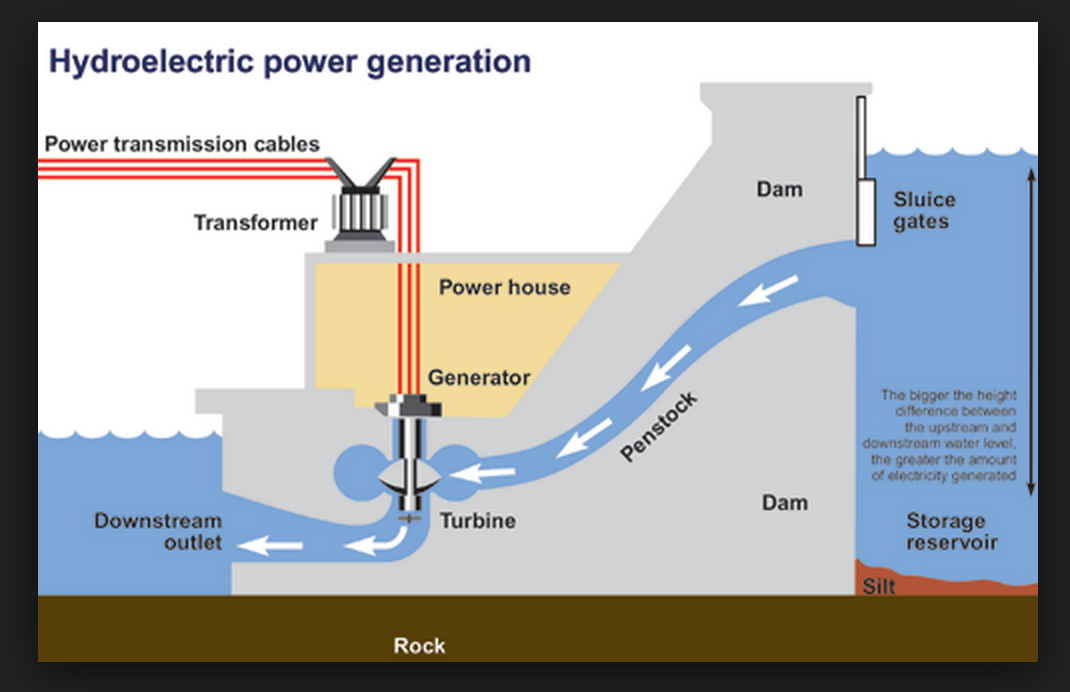
\includegraphics[width=1\textwidth]{hydro}
    \caption[Hydro Cycle]{Hydro Cycle \cite{Hydro}}
  \end{center}
\end{figure}

\newpage

\section{Wind Power}

Wind power has maybe the least environmental impact out of all of the power sources. Opperating from wind currents to rotate giant blades that are connected by a series of levers and gears to the generator. Figure \ref{windmillWorkings} shows this process. The current is then fed down the shaft of the windmill and off to whereever needed. Once constructed, windmills essentially have no maintenance cost and are practically self-sustaining except for when breakdowns occur and maintenance is performed. 

Although windmills have minimal environmental effects, they have five noticeable drawbacks. The first drawback is that they produce tiny amounts of power compared to fossile fuels. The second drawback is that that in order to be effective windmills must be build it groups called wind farm and these take up large amounts of space compared to a single fossil fueled power plant. Third, windmills have been known to be a cause of death to birds. Fourth, humans that live around windmills are generally displeased with the appearance, noise and frequent shadows that they create. Finally, windmills are also costly to build and can only be placed in windy locations to make them worth building. 
\bigskip


\begin{figure}[hbt]\label{windmillWorkings}
  \begin{center}
    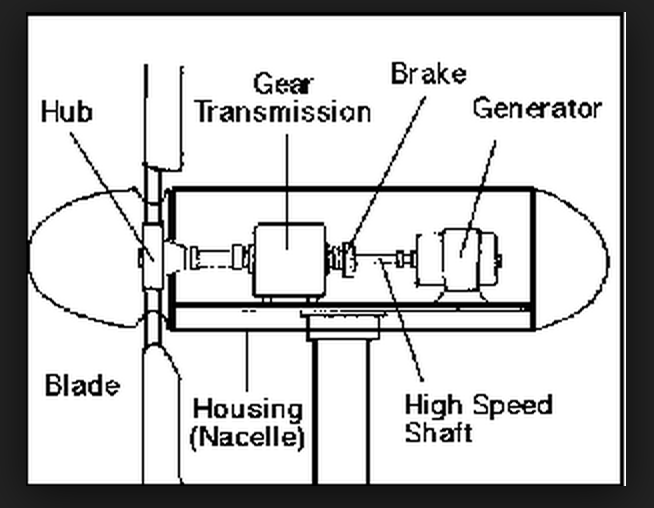
\includegraphics[width=1\textwidth]{windmill}
    \caption[Windmill Workings]{Windmill Workings \cite{Wind}}
  \end{center}
\end{figure}

\newpage

\section{Solar Power}
Solar power is the one power source that works in a completely different fashion from all of the others. When most objects are struck with rays of light, they absorb the incoming rays and convert this energy into heat. Solar panels are made from a special substance, primarily silicon. When this substance is struck with light it tends to react differently than most objects. When the electrons in solar panels are 
struck with light, they become excited and they raise an energy level. When enough electrons are at high enough energy levels they become loose and are able to move around. Electrons separate to the n (negative) type silicon and the protons remain in the p (positive) type silicon. In between the two types is a junction. This polarization of the two sides makes the loose electrons in the negative part of the panel able to move around. This motion forms a current in the cell and then the current can be redirected to where ever it is needed. Figure 
\ref{solarCell} shows this process. 

Solar panels have little to no maintenance cost and only require attention if they break down. They fit nicely on rooftops, and they have hardly any 
environmental impacts. Unfortunately, solar panels are the least efficient form of generating power, transforming  only about 20\% of the sunlight that hits them into usable electricity. In order to generate any significant amount of usable power, say enough to power amoderately sized population, farms of solar panels need to be built. This takes up huge amounts of space, far greater than any one fossil fueled power plant. With the increase of solar panals the cost also rises. Another drawback of solar panels is that they can only function during the day while the sun is up, which means that another source of power is required for night time activities. 
\bigskip
\begin{figure}[hbt]\label{solarCell}
  \begin{center}
    \includegraphics[width=1\textwidth]{Solar2}
    \caption[Solar Cell Workings]{ Solar Cell Workigns \cite{Solar}}
  \end{center}
\end{figure}


\section{Summary}

\begin{table}[tbph]
\centering
\caption{Summary of pros and cons for each power source}
\label{table:Summary}
\begin{tabular}{|c|l|l|}
\hline
 & \multicolumn{1}{c|}{Pros} & \multicolumn{1}{c|}{Cons} \\ \hline
Fossile Fuels & \begin{tabular}[c]{@{}l@{}}* Produces large amounts \\    of power\\ \\ \\ * Fuel is cheap to obtain\\ \\ \\ * Can be built close to cities\end{tabular} & \begin{tabular}[c]{@{}l@{}}* Fuel is finite\\ \\ \\ * Pollutes the environment\\ \\ \\ * Disrupts marine wildlife\end{tabular} \\ \hline
Nuclear & \begin{tabular}[c]{@{}l@{}}* Produces large amounts \\    of power\\ \\ * Fuel is abundant\\ \\ * Produces lower waste\\    than fossil fuels\end{tabular} & \begin{tabular}[c]{@{}l@{}}* Produces radio active \\    waste\\ \\ \\ * Disrupts marine wildlife\\ \\ \\ * Fuel is finite\end{tabular} \\ \hline
Wind & \begin{tabular}[c]{@{}l@{}}* Fuel source is infinite\\ \\ \\ \\ * Produces clean energy\\ \\ \\ \\ * Minimal environmental \\    effects\\ \\ \\ \\ * Low maintenance cost\end{tabular} & \begin{tabular}[c]{@{}l@{}}* People don't like living \\    near windmills\\ \\ \\ * Produces small amounts \\    of power\\ \\ \\ * Must be build in groups\\     to be effective\\ \\ \\ * must be built in windy \\    locations\end{tabular} \\ \hline
Solar & \begin{tabular}[c]{@{}l@{}}* Fuel source is infinite\\ \\ * Produces clean energy\\ \\ * No Environmental effects\\ \\ * low maintenance cost\\ \\ * Integrates well in cities\end{tabular} & \begin{tabular}[c]{@{}l@{}}* Weakest power source \\     at creating  power\\ \\ * Must be built in groups \\    to be effective\\ \\ * Can only work during \\     the day\\ \\ * Costly to build\end{tabular} \\ \hline
Hydro & \begin{tabular}[c]{@{}l@{}}* Fuel source is infinite\\ \\ * Produces clean energy \\    once built\\ \\ * Can produce large \\    amounts of energy\\ \\ * Can run all day and night\end{tabular} & \begin{tabular}[c]{@{}l@{}}* Huge environmental \\    cost to build\\ \\ \\ * Dams can be costly \\    to build\\ \\ \\ * Have to be built by \\    water\end{tabular} \\ \hline
\end{tabular}
\end{table}



\chapter{The Source}

The design of the system, as illustrated in figure 3.1 below, is straightforward. The user interacts with 
the system by purchasing power plants. This is done on a designated screen when there is land for the user 
to build on. Once the user has picked a type of power he/she must then provide the resources necessary for 
the power plant to function. The user can obtain fossil fuels by mining for them on the screen designated 
to represent the land that is currently available for the user to excavate. Once resources have been 
obtained and a power plant is built, energy can then be created and supplied to the population.
\bigskip

\begin{figure}[hbt]
  \begin{center}
    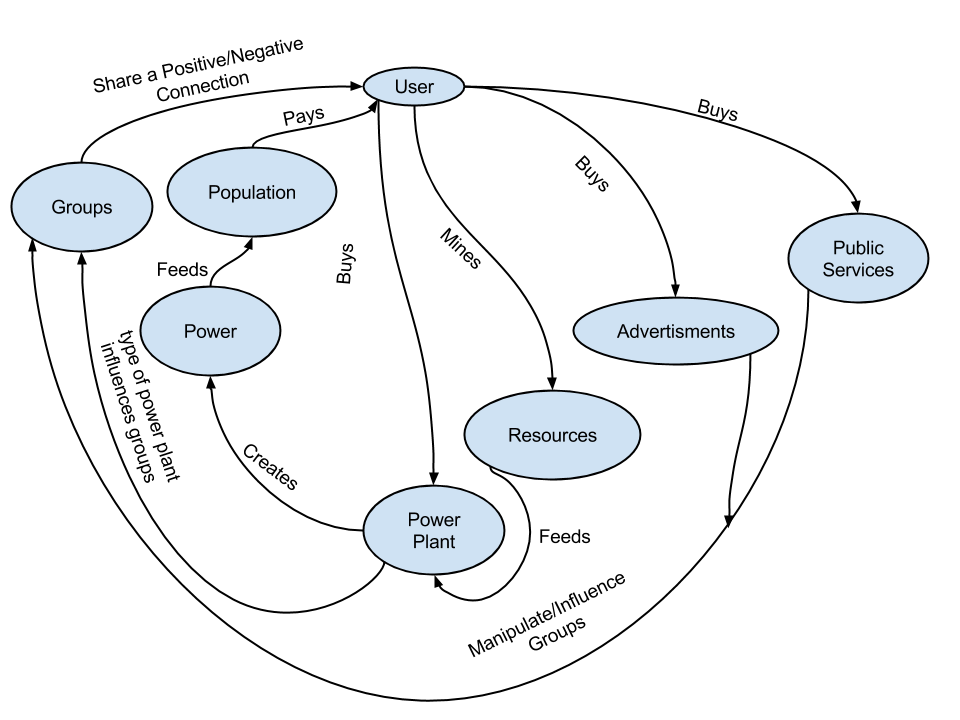
\includegraphics[width=0.9\textwidth]{DFDDiagram}
    \caption[Figure 1]{\label{DFD Diagram} }
  \end{center}
\end{figure}


Another option that the user has is that he/she can purchase advertisements or public services to help 
him/her flourish in the simulation. For example, a user could purchase an advertisement that educates the 
population to not waste power. This advertisement would reduce the usage of power and allow the user to 
more easily meet the demand. Users can also buy public services. An example would be a geologist that would 
survey the land and tell the user where to mine for a specific resource. Both of these purchases can 
influence groups within the game, such as environmentalists or public opinion. 
\bigskip


Users choices in the game affect groups as well, for example if a user invested in coal fueled power plants then the environmentalists group would not be displeased. Groups provide small perks or punishments to the user, usually in the form of grants or fines, which are dependent on the users play style and choices within the simulation. 


\section{Screen Layout}
“The Source” is composed of 8 different screen. The first five mentioned below are know as the five core screens. You can get to any of these screens from any other screen in the game. 
\bigskip

\noindent \large \textbf{ The Business Screen (one of the five core screens):} \newline
\indent In this screen the user is able to purchase advertisements and pubic services to help him/her 
progress through the simulation. Here the user is also able to see their progress throughout the game. The 
user will be able to see data like, money and energy made over time.  
\bigskip

\noindent The City Screen (one of the five core screens): \newline
\indent Here the user is able to see how the population is doing, the amount of power currently demanded and the amount supplied. This screens purpose is to purely display information.
\bigskip

\noindent The Power Plant Screen (one of the five core screens): \newline
\indent This screen, possibly the most education screen shows the workings of each type of energy as well as the inner workings of a generator. As well as seeing this information this screen allows the user to 
see specifics on the current power plants that he/she has built. Specifics being information such as 
amount of power produced, cost to maintain, resources required to maintain and more. 
\bigskip

\noindent The Land Screen (one of the five core screens): \newline
\indent From this screen the user can build power power plants that run off of fossil fuels and uranium. The user will have some designated land to start but he/she also has the option to buy more land to build 
on if the starting land is all used up.
\bigskip

\noindent The Resource Screen (one of the five core screens): \newline
\indent The purpose of this screen is to act like a map for the resources at the users disposal. From this 
screen the user can see all the resource that will be needed and the user can get at the three resource 
screens that will allow the user to extract the resources.
\bigskip

\noindent The Hydro Screen: \newline
\indent From here the user can view numerous rives that could be damned in order to generate power. Once a 
river is damned it will be shown on the screen. Rivers can only be damed once. 
\bigskip

\noindent Solar/wind Power Screen: \newline
\indent This screen shows land in the form of a grid that the user has at his/her to build windmills on or 
solar canals. Building will have a cost. Once something is built it can be dismantled to open the land 
to have something else built. 
\bigskip


\noindent The Fossil Fuels Screen: \newline
\indent Here land that the user can mine will be shown. This will be one large grid that will hold all the 
fossil fuels and uranium. The user can mine a section by selecting it and he or she will have a chance 
of discovering any one of the four resources. The resource discovered will go towards fueling the built 
power plants. Once a section is mined it can not be reused. 
\bigskip

\noindent The Static Screen: \newline
\indent The static screen is not really a screen at all but a combination of static images that remain on 
top of all other screens for the entire duration of the game. This serves as the means of navigation 	
between the five core screens. As well as displaying some information such as money and time. 
\bigskip

%Include citations in your thesis as you write:
%\cite{MR2848848,MR2461448,MR2834159,infconv,convmono,MR2668638,Bauschke:2007-PA02,proxbas}

%\section{Packages}
%There are several packages\ . So before you add a new package, check first if it is already included there.


%\section{Epigraph}
%If you want to add an epigraph to a chapter (epigraph in the sense of a literary inscription, not a function epigraph), you can use the command \texttt{epigraph} after the chapter. Check out the documentation of the \texttt{epigraph} package for more information.

% The following are examples of how to incorporate graphics into your thesis.

% \begin{figure}[ht]
%   \begin{center}
%     \includegraphics[width=0.4\textwidth]{figure}
%     \caption[Sample figure.]{\label{fig:happy} This is a sample figure
%       Note that we have
%       used the optional argument for the caption command so that only
%       a short version of this caption occurs in the list of figures.}
%   \end{center}
% \end{figure}

% \begin{figure}[ht]
%   \begin{center}
%     \includegraphics[width=0.4\textwidth]{figure}
%     \caption{\label{fig:happy2} This is the same sample figure with still
% 			a long caption but this time we did not use a short caption command
% 			in the table of figures.}
%   \end{center}
% \end{figure}

% You should really put text in between figures so LaTeX has more flexibility to place the figure at the appropriate location.



\chapter{Data Analysis}

\indent Over the course of a week and a half, 17 university students participated in testing using the method described in the last chapter. The original estimates of the timing of the testing were accurate. The amount of time taken to learn the game and the level of enjoyment did vary between people so the testing periods lasted from about 50 minutes to an hour and a half. In the following sections the results of the tests will be discussed and a conclusion will be reached as to whether or not ``The Source'' was educational and successful in being a positive playing experience.

\section{The Numerical Results}
As mentioned in the previous chapter, this questionnaire's purpose was to allow the user to express his or her thoughts, ideas, experiences and opinions on playing the game. Three different areas that were directly focused were the usefulness of items in the game, the difficulty of the game, and the users' playing experiences. 

\subsection{Usefulness}
\indent The first thing that required feedback was the usefulness of items in the game. The public services, power sources, and advertisements in the game allow for many different tactics and it is important to know users' decisions concerning all three of these items. The charts in figures \ref{powerSources}, \ref{ads} and \ref{publicServices} show the users' responses when asked why they did not purchase elements from a section.
 
\begin{figure}[hbt]
  \begin{center}
    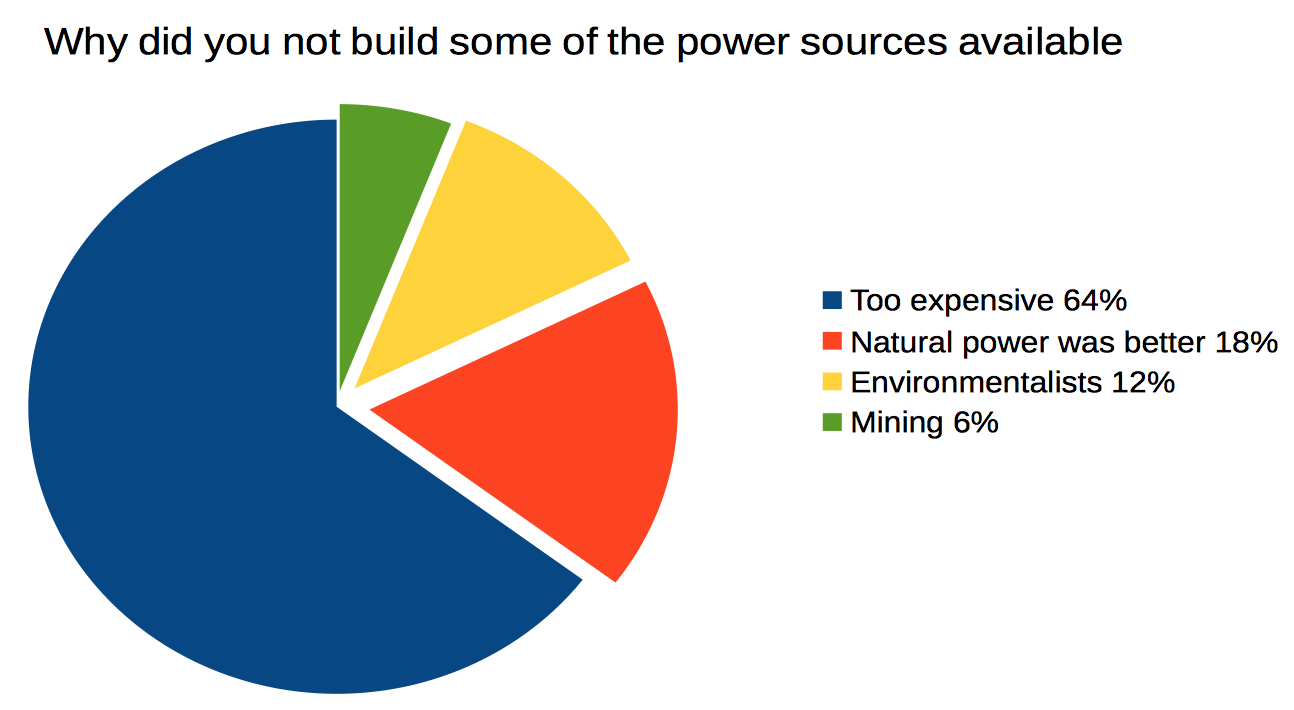
\includegraphics[width=1\textwidth]{survey_pics/numeric/power_source}
    \caption[Power Source Choices]{Power Source Choices}\label{powerSources}
  \end{center}
\end{figure}

\begin{figure}[hbt]
  \begin{center}
    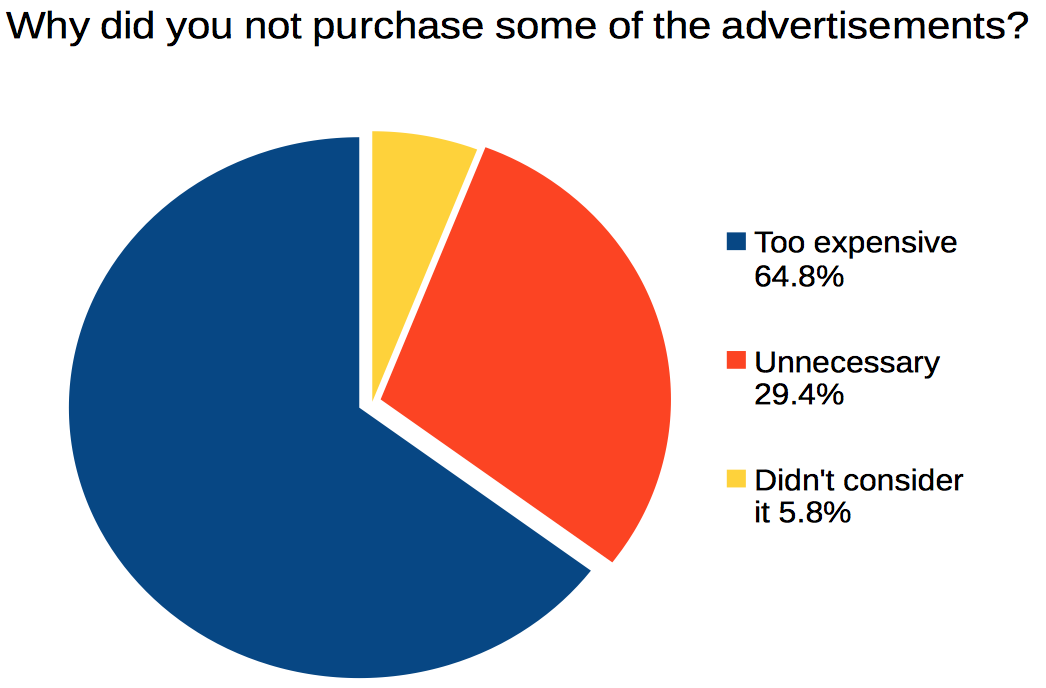
\includegraphics[width=1\textwidth]{survey_pics/numeric/adds}
    \caption[Advertisement Choices]{Advertisement Choices}\label{ads}
  \end{center}
\end{figure}

\begin{figure}[hbt]
  \begin{center}
    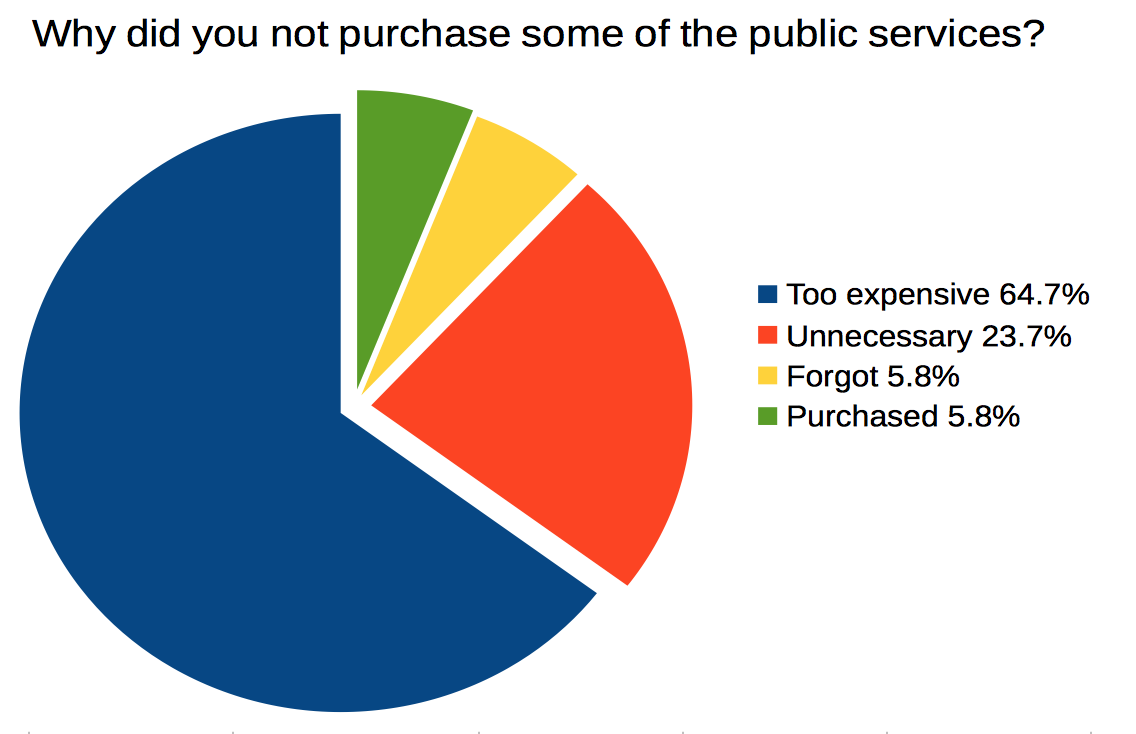
\includegraphics[width=1\textwidth]{survey_pics/numeric/public_service}
    \caption[Public Service Choices]{Public Service Choices}\label{publicServices}
  \end{center}
\end{figure}

\newpage
In all three charts, the main reason why users didn't purchase items was because of the cost. Users evaluated the cost of the items and deemed them not worthy of the time and money required. Having this many people come to this conclusion shows that the cost of the items should be reduced to allow users to feel that they have more choices.

Nearly 30\% of people came to the conclusion that advertisements were an unnecessary investment. This is nearly a third of the poplulation which suggests that the perks that groups give should be reconsidered to give more positive advantages to the user rather than just preventing disadvantages. 17\% of people came to the same conclusion about public services; that public services posed no real advantage. However, the data monitored by the system shows that the few people who managed to invest in them were able to thrive for a while off of the perks provided by the public services. While it can be said that some people saw public services as a waste, some people saw an opportunity, and hence public services cannot be claimed as positive or negative for certain with so many participants being scared off by the price. 

17\% of participants said that natural power was a better investment and although this number is influence by the price of the other power sources, it does suggest the possibility that maybe natural power is too strong. Natural power was meant to help the user get started in the early stages of the game and then fall off later but many users developed the strategy of investing into natural power for as long as possible. 

\newpage
\subsection{Difficulty}
\indent Another area that needed investigating was the difficulty that the user experienced while playing the game. Of interest to know was if the user had too easy or too difficult of a time playing. The game should not be so simple as to be mindless but should not be too difficult as to make the user give up. This difficulty was evaluated in three different questions, how difficult the user found it to keep up with demand, how the user thought the pace of the game was, and if the user found some items to be too expensive or too cheap. The results of each question are shown in figures \ref{powerDemanded}, \ref{gamePase} and \ref{cost}.
\bigskip
\newpage
\begin{figure}[hbt]
  \begin{center}
    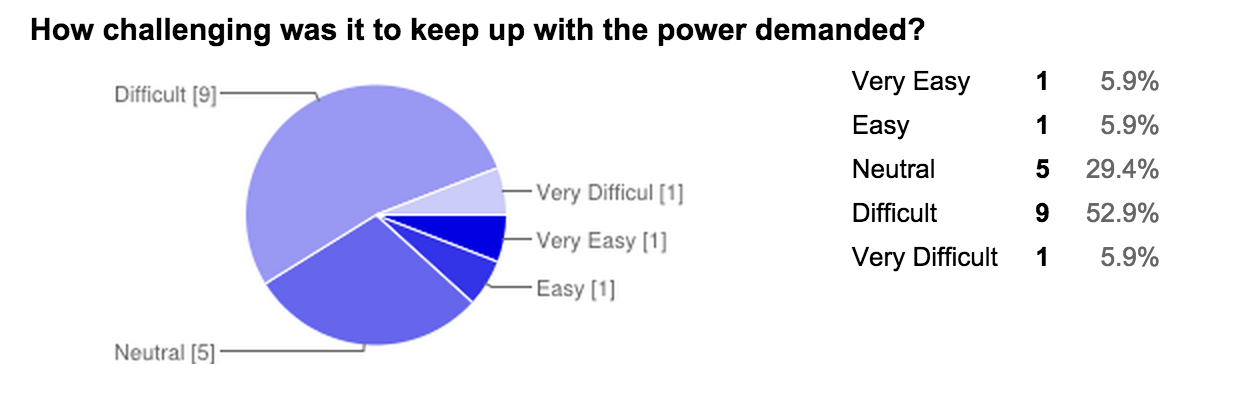
\includegraphics[width=1\textwidth]{survey_pics/numeric/power_demanded}
    \caption[pd]{Power Demand Difficulty Level}\label{powerDemanded}
  \end{center}
\end{figure}

\begin{figure}[hbt]
  \begin{center}
    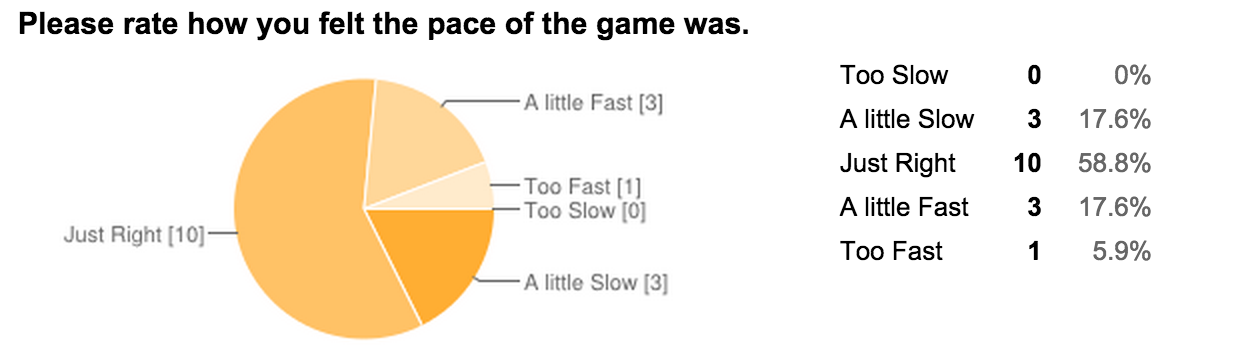
\includegraphics[width=1\textwidth]{survey_pics/numeric/game_pase}
    \caption[p]{Game Pase Rating}\label{gamePase}
  \end{center}
\end{figure}

\bigskip
\begin{figure}[hbt]
  \begin{center}
    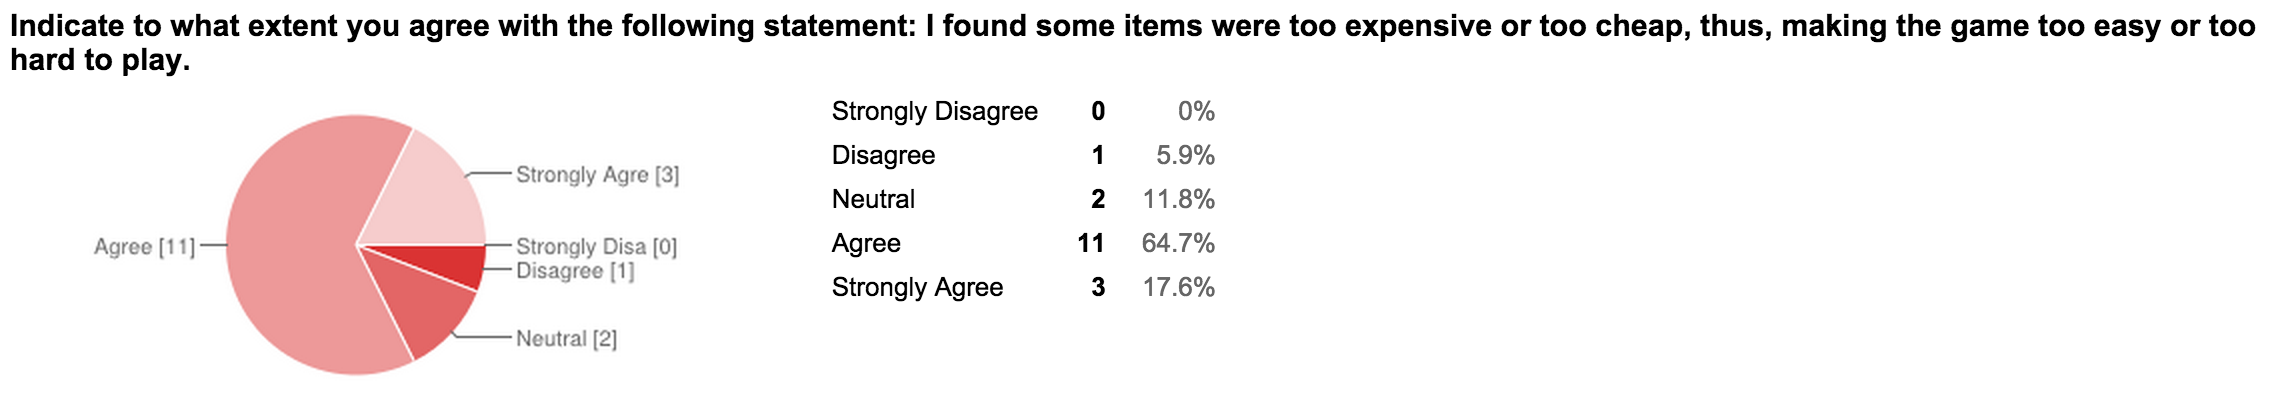
\includegraphics[width=1\textwidth]{survey_pics/numeric/cost}
    \caption[Power Source ]{Expensive/inexpensive items}\label{cost}
  \end{center}
\end{figure}

As can be seen in figure \ref{powerDemanded} the majority of the pariticipants had a difficult time keeping up with the power demanded and this is to be expected, however, the game is intended for a younger audience. If university students had a difficult time keeping up it is reasonable to believe that high school students should have even more of a challenge. This issue could be resolved by lowering the cost of the items that the users had already believed were too expensive.

Figure \ref{gamePase} shows that a majority of participants were able to cope with the pace of the game. This data shows that the pace of the game is probably not a big factor in the difficulty of the game. 

\newpage
In figure \ref{cost} the data indicates that nearly every participant found that the cost of items could use revising. In follow up questions the users said that almost all of the items and all of the non-natural power sources cost too much. This additional cost added a great deal of financial difficulty to the game. Not being able to purchase power plants is the main way that the game should show its difficulty but it can not be the only way. If purchasing power plants was the only obstacle then the user would only have to face this one problem every time he or she played. Instead the user should be facing a price obstacle as well as many other smaller obstacles created by the choices the user makes while playing. From the users' responses it can be determined that financial difficulty needs to be decreased and replaced in other sections of the game. This modification will create a more dynamic game every time the user plays, which will in turn make the game more interesting.



\subsection{Playing Experience}
\indent The previous two sections were dedicated to discovering potential flaws that lay within the framework of the system, but the game's core goal to provide a positive playing experience to the user must also be investigated. To see if ``The Source'' was sucessful the users were asked to comment on their frustration, playing experience, learning, mis-click, rate and tutorial experience. Out of curiosity, the user was also asked if he or she was motivated to research power on his/her own time. The results of these questions are just below in figures \ref{frusterated}, \ref{playingExperience}, \ref{learning}, \ref{mis-click}, \ref{tutorial} and \ref{future_learning}. 



\begin{figure}[hbt]
  \begin{center}
    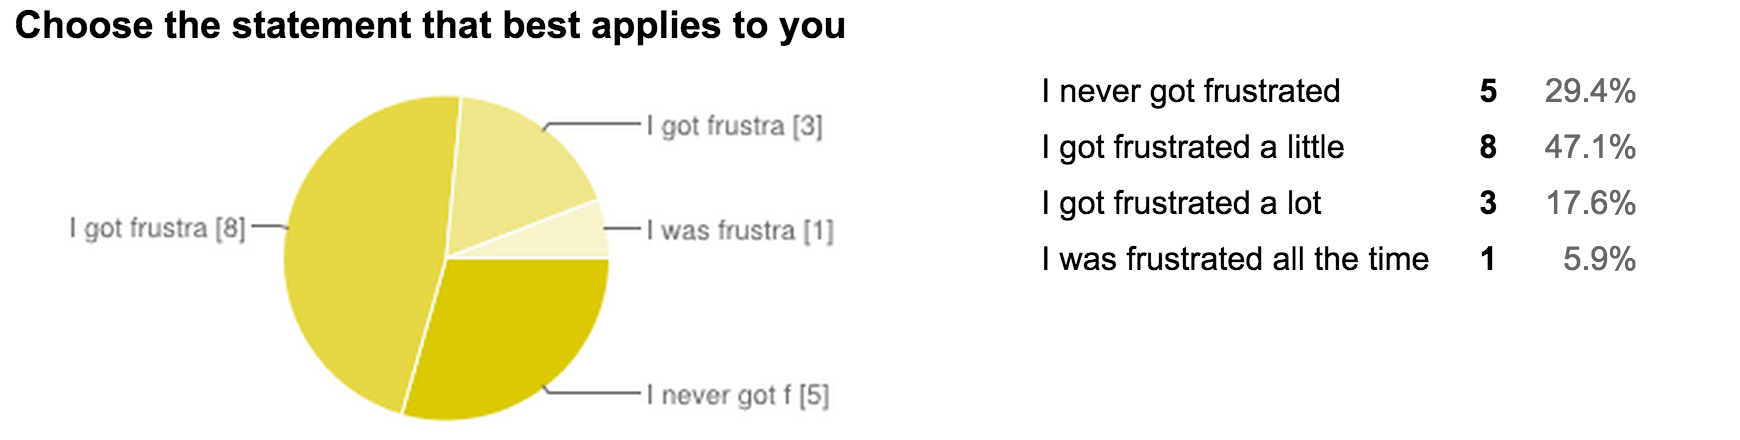
\includegraphics[width=1\textwidth]{survey_pics/numeric/frusterated}
    \caption[Frustration Levels]{Frustration Levels}\label{frusterated}
  \end{center}
\end{figure}



\begin{figure}[hbt]
  \begin{center}
    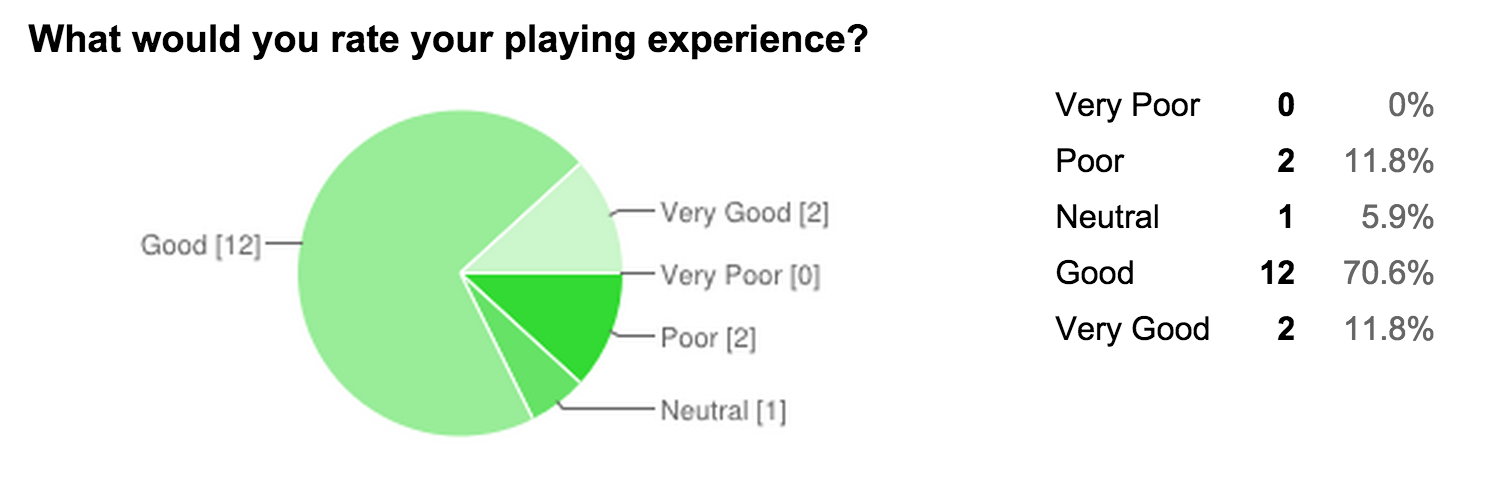
\includegraphics[width=1\textwidth]{survey_pics/numeric/playing_experience}
    \caption[Playing Experice Rating] ]{Playing Experience Rating}\label{playingExperience}
  \end{center}
\end{figure}


\begin{figure}[hbt]
  \begin{center}
    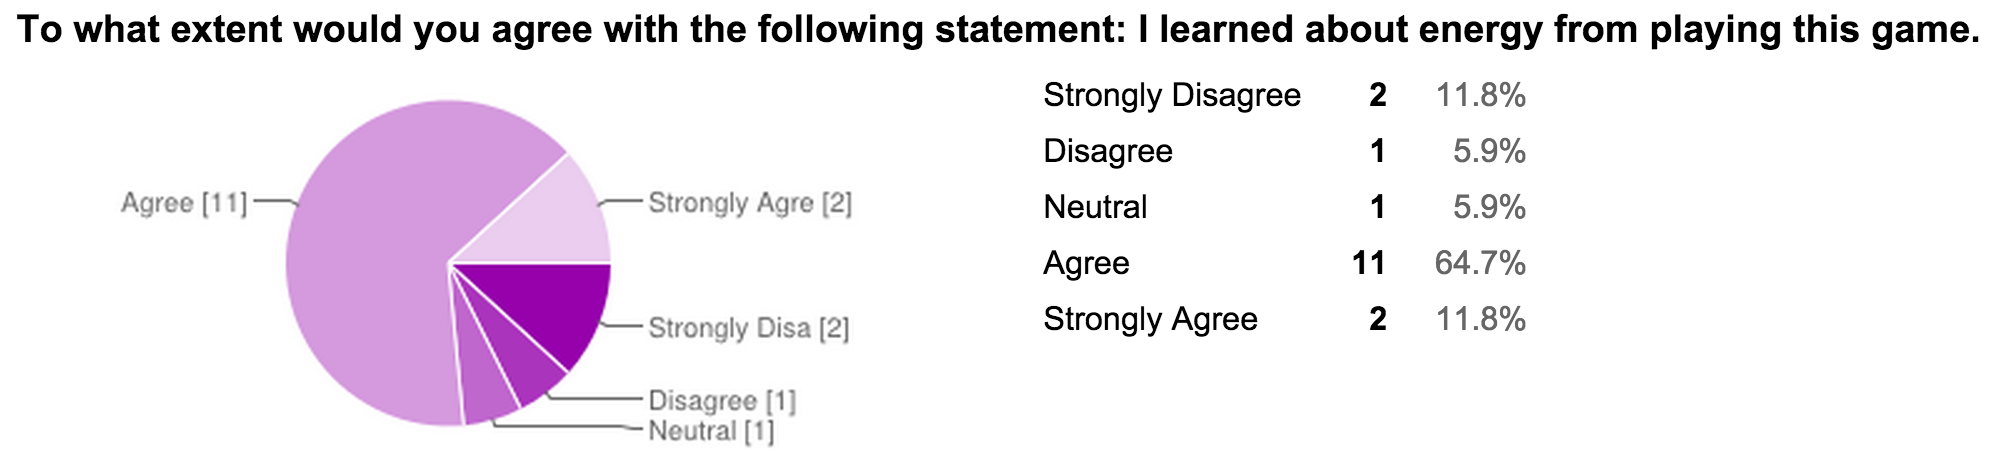
\includegraphics[width=1\textwidth]{survey_pics/numeric/learning}
    \caption[Learning level ]{Learning Level}\label{learning}
  \end{center}
\end{figure}


\begin{figure}[hbt]
  \begin{center}
    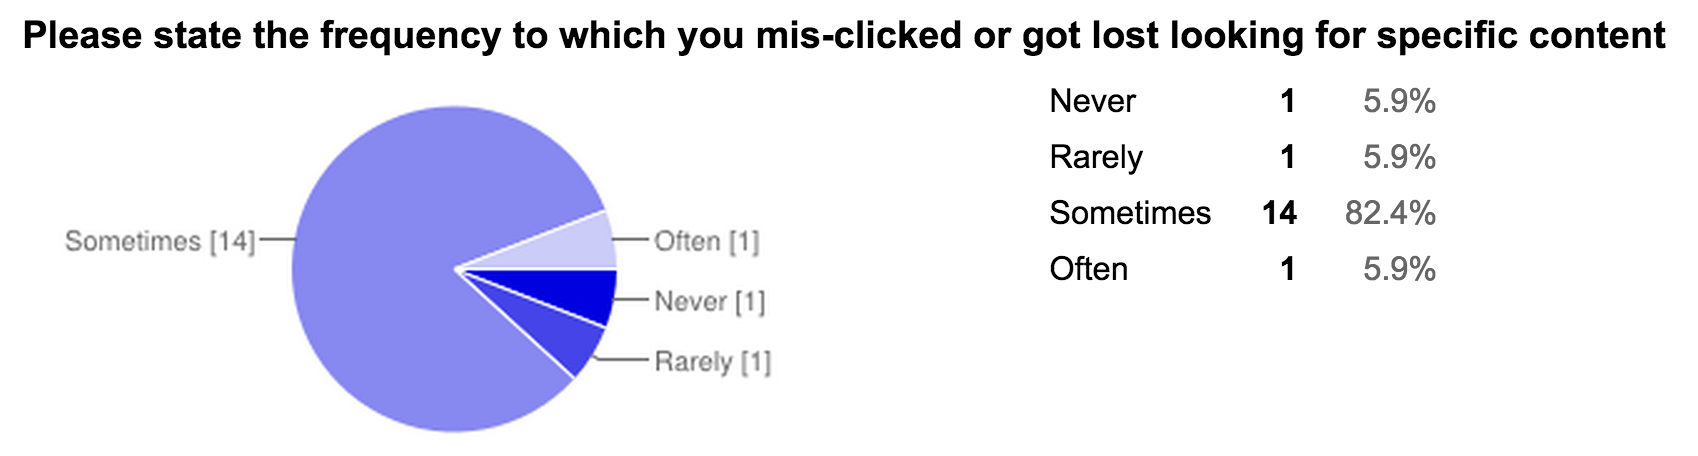
\includegraphics[width=1\textwidth]{survey_pics/numeric/mis_clicked}
    \caption[Mis-Click Rate ]{Mis-Click Rate}\label{mis-click}
  \end{center}
\end{figure}


\begin{figure}[hbt]
  \begin{center}
    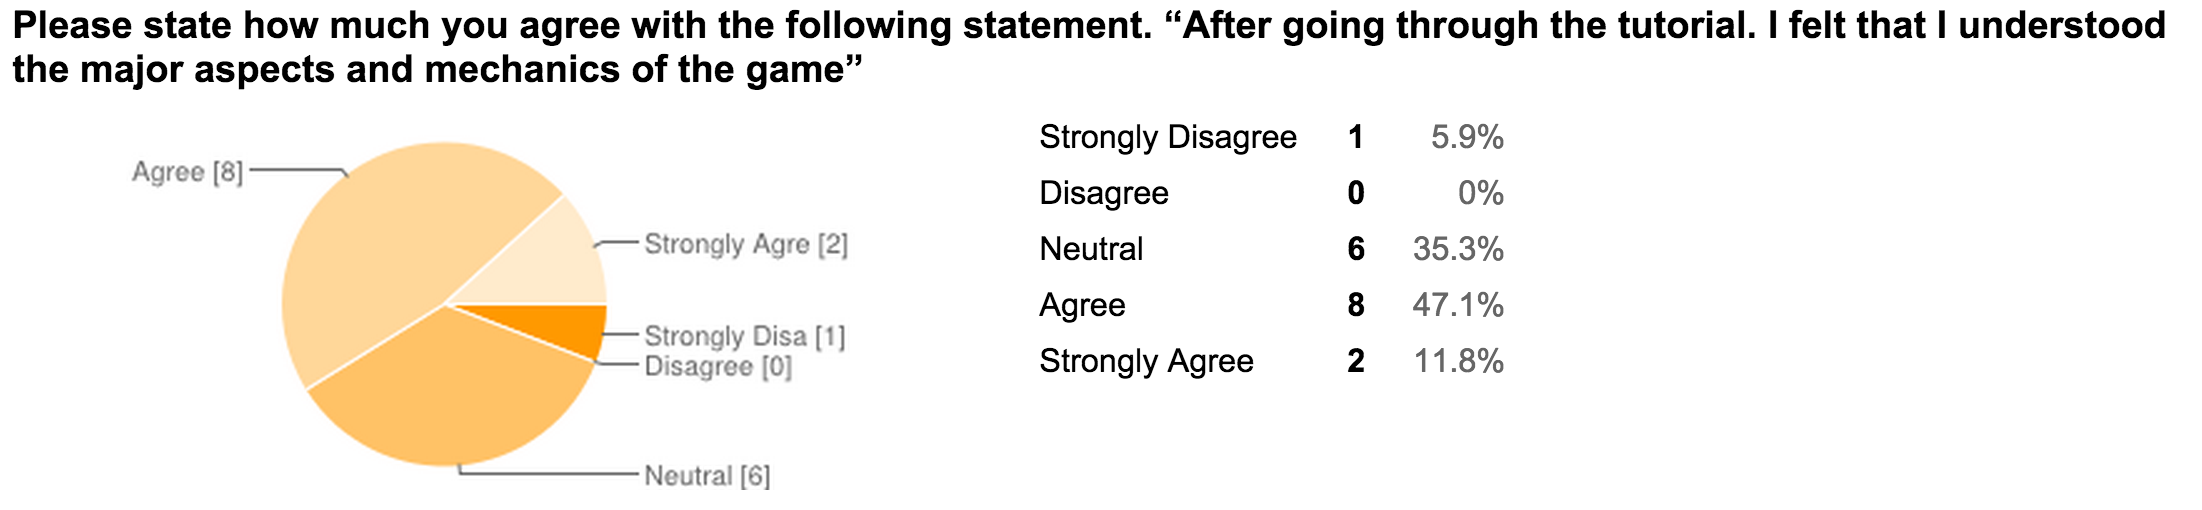
\includegraphics[width=1\textwidth]{survey_pics/numeric/tutorial}
    \caption[Tutorial Experience]{Tutorial Experience}\label{tutorial}
  \end{center}
\end{figure}

\begin{figure}[hbt]
  \begin{center}
    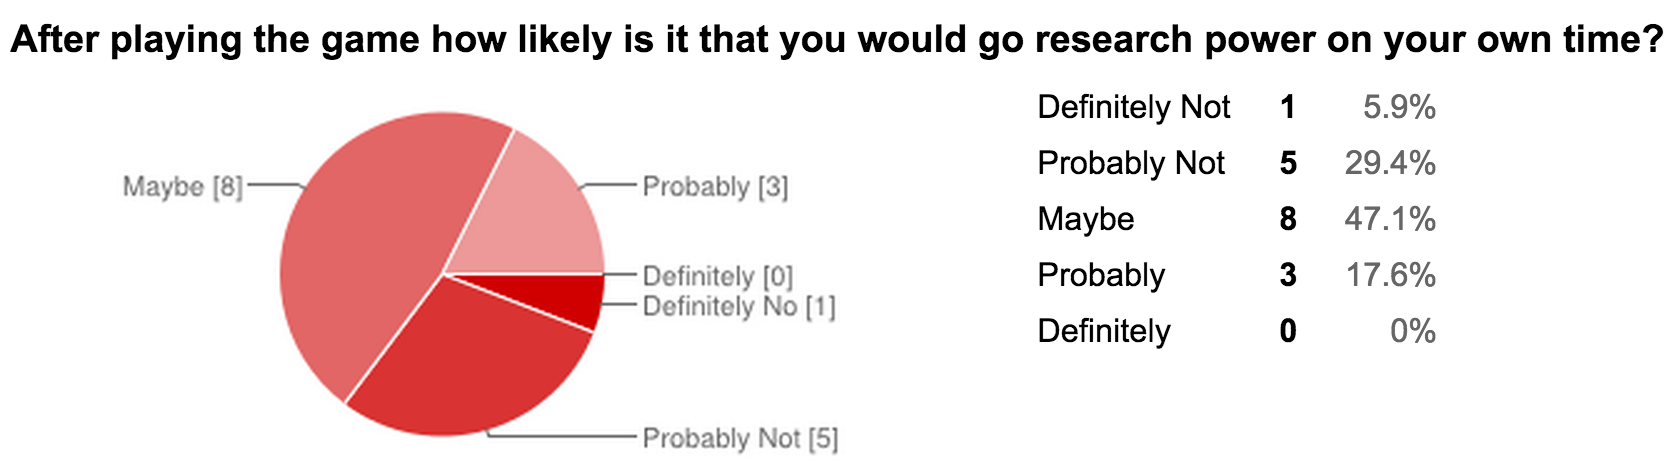
\includegraphics[width=1\textwidth]{survey_pics/numeric/future_learning}
    \caption[self Learning ]{Likelihood Of Self Research}\label{future_learning}
  \end{center}
\end{figure}


Clearly, figure \ref{frusterated} shows that the majority of the users fell within the acceptable range of experiencing little or no frustration. The game is fairly large and has multiple screens for dedicated tasks, and as such it was expected for some participants to experience high levels of frustration especially if they rushed through the lengthy tutorial.

From figure \ref{playingExperience} it can be seen that over 80\% of the participants had a positive experience playing which is important to maintain user interest and attract new users.

Figure \ref{learning} shows that over 75 \% of participants felt that they learned something about energy while playing this game. This data is an excellent indication of success in the other core goal of ``The Source'', which is educating the user about energy. This data is further explored in the following section.

From the data in figure \ref{mis-click}, which is directly related to the user's frustration level, it is expected to see a relation between user mis-clicks and user frustrration. However this data is not indicative of a clear conenction. This data shows that the game has other frustrating aspects, which other data indicates may possibly be the financial difficulty that most people experienced.

It can be seen in figure \ref{tutorial} that the tutorial was successfull in its task of informing the user of his/her objectives and the mechanics of the game. After completing the tutorial, over 90\% of participants felt ready to take on the game. Although this percentage is excellent, almost all of the participants mentioned that the tutorial was too long and that they tried unsuccessfully to use the tutorial as if it were interactive, which it was not. Although the tutorial performed its task for this study it is unlikely that it would be effective in the real world as the attention span of users would not be long enough.

The other core goal of ``The Source'' is to educate the user on how the main sources of energy function, but there is too much information and detail to fully explain each power source in detail. ``The Source'' merely opens the door and gives user a taste as to what is out there, and hopefully inspires people to research a little more into power on their own time. Figure \ref{future_learning} shows that \percent{11}{17} of participants showed potential in researching power on their own time. 


All of the data collected from the playing experience section of the usability study indicates that the users had positive playing experiences and the game was user friendly. This positive outcome means that ``The Source'' has successfully met its usability goals. In fact, the majority of the data collected for each question in this section has a positive outcome.  

\section{Knowledge Test Results}
\indent The purpose of the knowledge test was to discover if the user had learned anything during the game. As mentioned before a pre and post-test method was used to compare users' knowledge before and after playing ``The Source''. ``The Source'' can claim to be successful if more people get the right answer in the post test than the pre test. The knowledge test will be discussed in two parts; first, the operation section which covers how power plants operate, and second, the pros/cons section which covers the pros and cons of each power source. These two pieces are broken up because the information involved was presented to the users in two different ways.


\subsection{Operation of a Power Plant}
    In both the pre and post-tests users were asked about the general idea of how each kind of power opperates and the idea behind modern generators. Within the game lies a screen with small (10-20) animations about how each type of power operates. Users are almost guaranteed to see each animation as they are instructed to explore the game on their first attempt at playing. Each animation holds the answer to the relavent question asked in the questionnaire. The results of the question are shown in figure \ref{workings}. The graph shows that there was an increase in knowledge in almost all areas except nuclear and coal power. Knowledge in nuclear power remained the same, which suggests that people didn't visit the screen where the nuclear power knowledge was presented. This relationship agrees with what a few users mentioned, that the game forced the user to care about coal more than the other non-natural power sources, because the user starts off with a coal power plant. In future work the user could start off with a random power source so they are forced to see all knowledge screens. Figure \ref{workings} also shows that one person did worse after playing the game when asked about the workings of coal power plants. Reasons why this decreased occurred are unknown and should not have happened for a number of reasons. First, since users start with a coal power plant they are almost guaranteed to visit the screen that presents them with the knowledge of how coal power plants operate. The information is not hidden or avoidable, if the user visited this screen he or she would have had to have seen it. Secondly, users showed an improvement in both gas and oil power plants which work the same way as coal power plants. If the user knows how one operates he or she knows how the other three operate as well. 
    Even with this one anomaly, looking at the data as a whole it is clear that in all of the other categories of power there was an increase of correct answers after playing the game. This increase demonstrates that ``The Source'' is capable of teaching users about energy. 


\begin{figure}[hbt]
  \begin{center}
    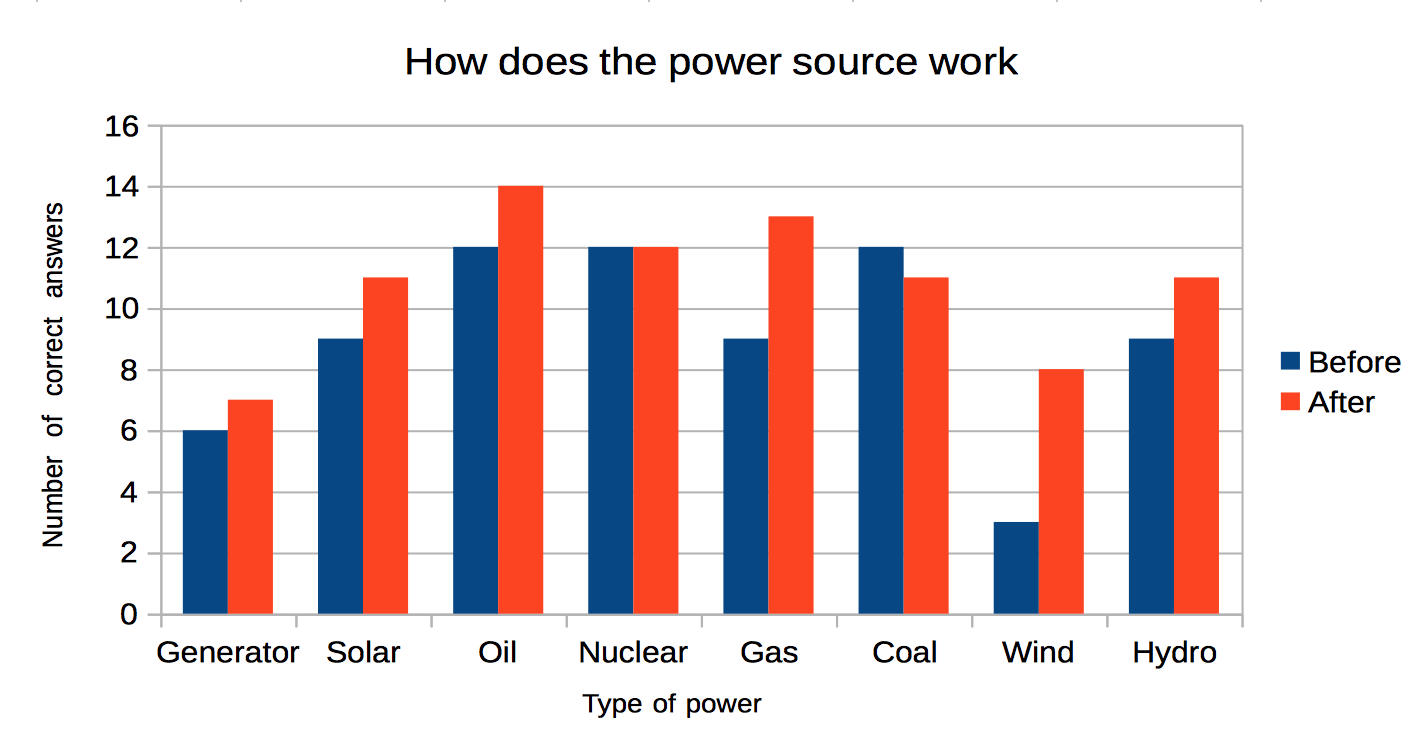
\includegraphics[width=1\textwidth]{survey_pics/post_and_pre/workings}
    \caption[Working Powerplants ]{Correct answers to the workings of a power type}\label{workings}
  \end{center}
\end{figure}

\subsection{Origins of Power}
  In this section of the questionnaire users were asked where the fuel sources of each type of power came from. In these questions solar power was ignored due to its simplicity. In the case of wind and hydro the questions focussed more on what kinds of moving air and water fueled the power types. An example of a type of air would be ``rising air due to heat and oceans''. In the case of nuclear power the users were asked what fuels nuclear power and how the fuel is obtained. The answers to these questions were never dirrectly displayed to the user but instead they have to perform the action themselves. For example, coal is mined from the earth and in the game in order to obtain coal and other fossil fuels, users had to mine sections of land. In the case of natural power the answers were shown in the animated videos because you can not create or purchase sunlight, water, or moving air. The results of this question are shown in figure \ref{origins}. The graph shows that at least one person showed improvement in all aspects of power. The graph clearly shows that users increased knowledge in this area.

  \begin{figure}[hbt]
  \begin{center}
    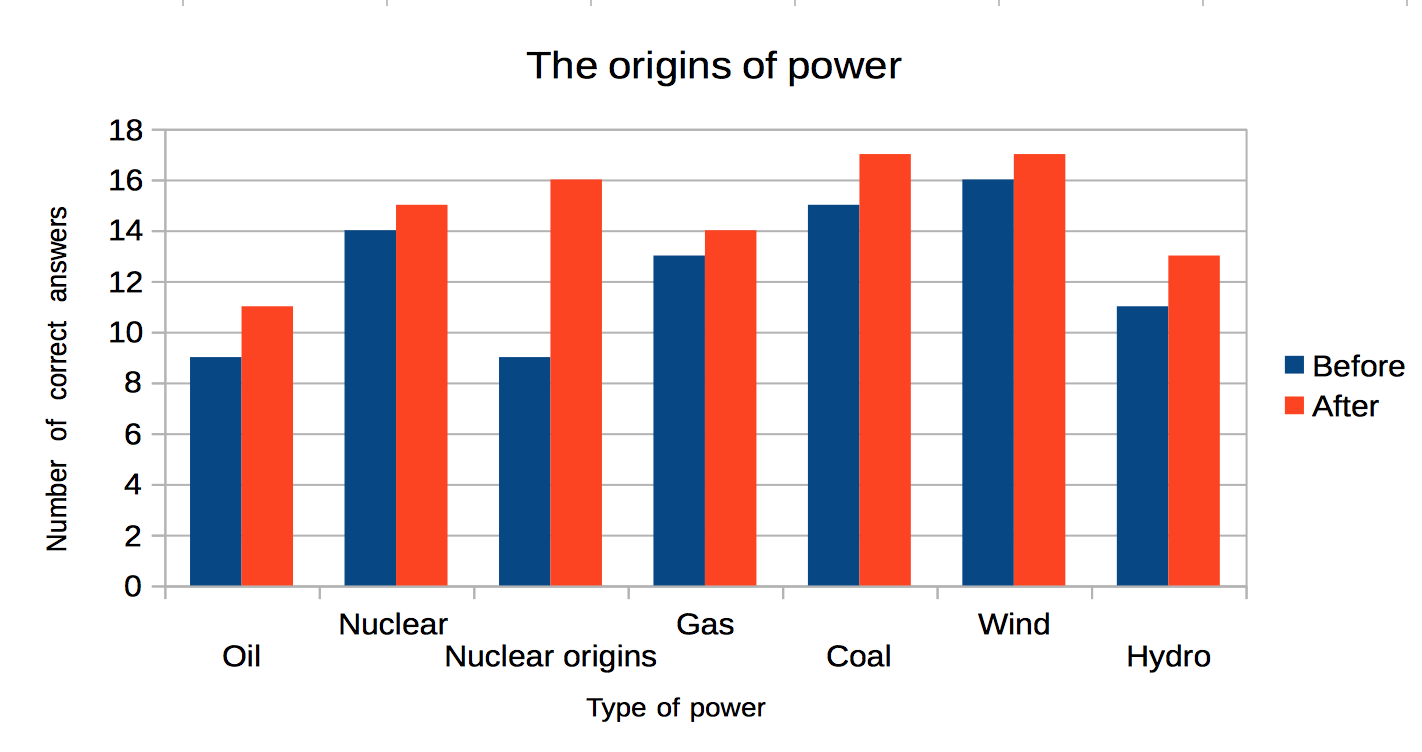
\includegraphics[width=0.8\textwidth]{survey_pics/post_and_pre/origins}
    \caption[Origions of power fuel]{Correct answers to origions of power plant fuel}\label{origins}
  \end{center}
\end{figure}

\subsection{Pros and Cons}
In this section of the questionnaire users were asked to select a number of statements that they thought were advantages and disadvantages to the power source that the question was referring to. The answers to each question were located in the section of the game where the user would purchase a power source. This way the user could see the pros and cons of each power type before making a purchase. The results of the questionnaire are shown in figures \ref{pros} and \ref{cons}. The graphs are not nearly as clean as the others covered in the previous two sections. Here each graph has a few unexplainable flaws. The pros show that no pros were learned in 3 out of the 7 types of power and that some people for some reason did worse on 2 of the 7 power types. Even though the graph shows that at least two people improved on the remaining types of power, the negative data is too substantial to ignore. The cons graph is only marginally better than the pros. In 2 of the 7 types of power no progress was shown and people actually did worse when asked to list the cons of oil power plants. Even though some areas show an increase in knowledge the data overall is too weak to show an increase in knowledge. 

\indent There are a couple of possible reasons for this sudden shift in the data trends compared to the previous two sections which showed promising results. First, the answers to the questionnaire in this section were in text form. Meaning that the user had to read a segment of text while playing for each type of power to learn the pros and cons. Users are unlikely to read anything that they don't have to and since this text didn't contain vital information it is very likely that they could have given up on reading after the first sentence and hence not learned the information. Another reason is that users could have misinterpreted questions or answers on the questionnaire as some users asked for clarification on certain items. It is possible that some users had some questions about items but didn't ask which could have thrown off their answers.

\indent In summary, improvement was shown in the general understanding of how power sources operate and in the understanding of the origins of fuel for each power source. The pros and cons of power sources show no conclusive data to indicate one way or another if there was an improvemnt in the understanding of pros and cons or not. When looking at the data with the pros and cons data removed, it can be seen from the improvment in the first two sections that a majority of users were able to walk away having learned a few facts about the origins of power and the operation of power plant. 

\newpage
\begin{figure}[hbt]
  \begin{center}
    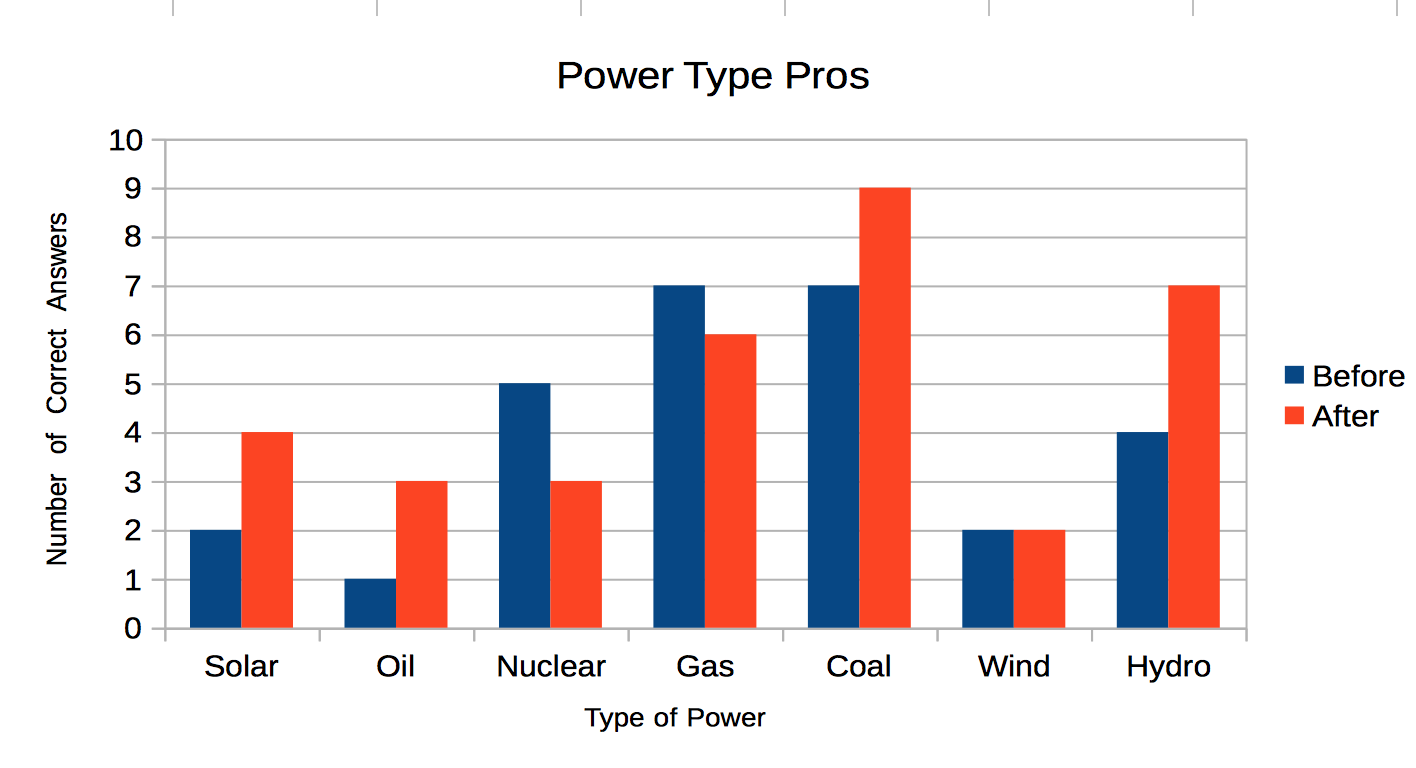
\includegraphics[width=0.8\textwidth]{survey_pics/post_and_pre/pros}
    \caption[Correct pros ]{Correct answers to pros of a power type}\label{pros}
  \end{center}
\end{figure}

\begin{figure}[hbt]
  \begin{center}
    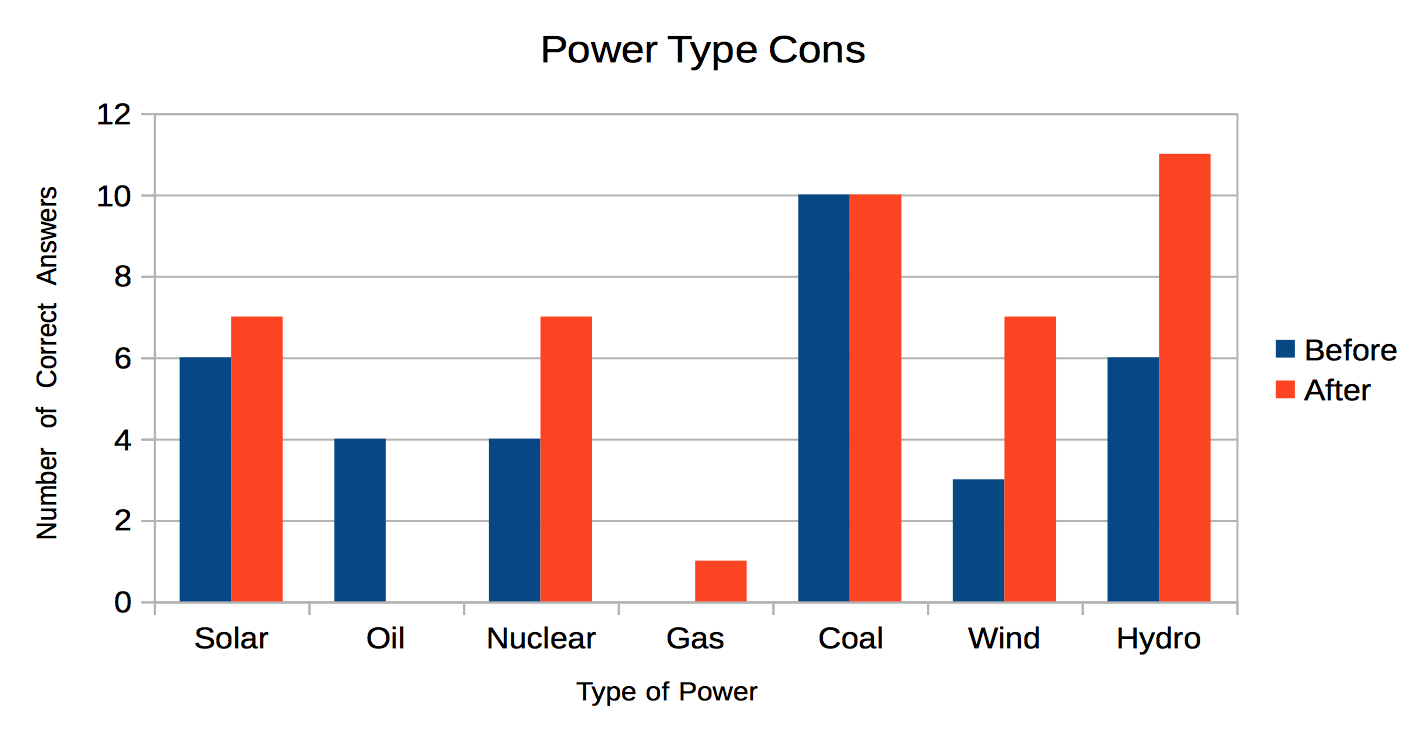
\includegraphics[width=0.8\textwidth]{survey_pics/post_and_pre/cons}
    \caption[Correct cons]{Correct answers to cons of a power type}\label{cons}
  \end{center}
\end{figure}

\newpage
\section{Conclusion}
From the data mentioned above and the conclusions met from each data set, it is clear that ``The Source'' was successful in providing the user with a positive playing experience and that ``The Source'' was able to teach its audience about the origins of power and the operation of power plant. Therefore, it can be said the the game has achieved both its usability and educational goals.


\chapter{Landscape Mode}
The landscape mode allows you to rotate a page through 90 degrees.  It
is generally not a good idea to make the chapter heading landscape,
but it can be useful for long tables etc.

\begin{landscape}
  This text should appear rotated, allowing for formatting of very
  wide tables etc.  Note that this might only work after you convert
  the \texttt{dvi} file to a postscript (\texttt{ps}) or \texttt{pdf}
  file using \texttt{dvips} or \texttt{dvipdf} etc.
\end{landscape}

\chapter{Conclusion}
Here comes the conclusion.

\begin{table}[tbph]
\centering
\caption{A publication quality table. Very very very very very very very very very very long title.
\label{table:food1}}
\begin{tabular}{@{}llr@{}} \toprule 
\multicolumn{2}{c}{Item} \\ \cmidrule(r){1-2} 
Animal & Description & Price (\$)\\ \midrule 
Gnat & per gram & 13.65 \\ 
& each & 0.01 \\ 
Gnu & stuffed & 92.50 \\ 
Emu & stuffed & 33.33 \\ 
Armadillo & frozen & 8.99 \\ \bottomrule 
\end{tabular}
\end{table}

\newpage
Your conclusion can go on for several pages.


% This file is setup to use a bibtex file sample.bib and uses the
% plain style.  Other styles may be used depending on the conventions
% of your field of study.
%
% Note: the bibliography must come before the appendices.


%change heading ``Chapter 5 Bibliography''->''Bibliography''
\newpage %newpage needed otherwise pagestyle applied to previous chapter. Does not actually create a new page
\pagestyle{fancy}\chead{Bibliography}\rhead{}\cfoot{}\rfoot{\thepage}

%Bibliography style is discipline dependent. Mathematic student can use e.g. SIAM
\bibliographystyle{ubco}
%\bibliographystyle{siam}
\bibliography{bibliography}%name of your .bib file

\newpage
\pagestyle{headings}
\addtocontents{toc}{%
\protect\renewcommand*\protect\cftchappresnum{\appendixname~}}

\appendix 
\addappheadtotoc %uses the current page number when it makes the entry in the ToC
\appendixpage 

\addtocontents{toc}{
\setlength{\cftbeforechapskip}{\cftbeforesecskip}
\setlength{\cftchapindent}{\cftsecindent}
\protect\renewcommand{\cftchapfont}{\cftsecfont}
\protect\renewcommand{\protect\cftchapdotsep}{\cftsecdotsep}
}


\chapter{Tables}
Here you can have additional tables. Table captions are always on top.

In order to use publication quality tables, one should use the guidelines in . In short, do not use vertical rules or double rules, units in the column heading (not in the body of the table), precede decimals with a digit, and do not use ditto signs. Table \ref{table:food} is according to the guidelines. 

For tables, the caption goes on top, for figures, the caption goes on the bottom. If possible, always position tables and figures at the top of a page.\footnote{In this case, the chapter heading prevents the table from being at the top.} Use the option \verb|tbph| for the placement.

\begin{table}[tbph]
\centering
\caption{A publication quality table. Very very very very very very very very very very long title.
\label{table:food}}
\begin{tabular}{@{}llr@{}} \toprule 
\multicolumn{2}{c}{Item} \\ \cmidrule(r){1-2} 
Animal & Description & Price (\$)\\ \midrule 
Gnat & per gram & 13.65 \\ 
& each & 0.01 \\ 
Gnu & stuffed & 92.50 \\ 
Emu & stuffed & 33.33 \\ 
Armadillo & frozen & 8.99 \\ \bottomrule 
\end{tabular}
\end{table}

\newpage
And other table materials (I needed to generate two pages for that appendix to test the formatting of the table of content).

\begin{table}
\caption{Another table}
\end{table}

\begin{table}
\caption{Another table}
\end{table}
\begin{table}
\caption{Another table}
\end{table}
\begin{table}
\caption{Another table}
\end{table}
\begin{table}
\caption{Another table}
\end{table}

\begin{table}
\caption{Another table}
\end{table}
\begin{table}
\caption{Another table}
\end{table}
\begin{table}
\caption{Another table}
\end{table}
\begin{table}
\caption{Another table}
\end{table}
\begin{table}
\caption{Another table}
\end{table}

\chapter{Figures}
Here you can have additional figures. Figure captions are always at the bottom.

\newpage

And other additional figures (again I needed to generate two pages :-).
% Indices come here.


\end{document}
\endinput
